\subsection*{Sistemas de N grados de libertad forzados}


\item Considere que en el sistema de dos péndulos acoplados del problema \ref{pendacop} y uno de ellos es impulsado por una fuerza $F= F_0 \cos(\Omega t)$.  
\begin{enumerate}
	\item Escriba las ecuaciones de movimiento del sistema con amortiguamiento y forzado, y desacople las ecuaciones utilizando las coordenadas normales del sistema.
	\item Resuelva el sistema forzado para las coordenadas normales. Escriba la solución más general posible para las coordenadas en el caso estacionario (pasado el transitorio).
	\item Estudie en el estado estacionario cuando las partículas están en fase o contrafase.
	\item Muestre que en el caso tienen $m_a= m_b= m$ si se  desprecia el amortiguamiento se obtienen las expresiones
	\[
		\begin{aligned}
			\Psi_a &\approx \frac{F_0}{2m} \cos(\Omega t) \left[ \frac{1}{\omega_1^2 - \Omega^2 } + \frac{1}{\omega_2^2 -\Omega^2} \right], \notag \\
			\Psi_b &\approx \frac{F_0}{2m} \cos(\Omega t) \left[ \frac{1}{\omega_1^2 - \Omega^2 } - \frac{1}{\omega_2^2 -\Omega^2} \right], \notag \\
			\frac{\Psi_b}{\Psi_a} &\approx \frac{\omega_2^2 - \omega_1^2}{\omega_2^2 + \omega_1^2 - 2 \Omega^2}, \notag
		\end{aligned}
	\]
	donde $\omega_1$ es la menor de las frecuencias modales, $\omega_2$ es la mayor y $\Omega$ es la frecuencia de excitación.
	\item (*) Grafique $\frac{\Psi_b}{\Psi_a}$, ¿qué representa esta relación?
	Indique cuándo hay una transferencia efectiva de movimiento y cuándo no.
\end{enumerate}


\item Considere el sistema del problema \ref{2masitas}, pero en este caso en considere las oscilaciones longitudinales.
\begin{enumerate}
    \item Halle la solución estacionaria para el caso forzado en el cual se aplica sobre la masa de la izquierda una fuerza oscilante $F(t)= F_0 cos(\Omega t)$.
		¿Qué resonancias espera ver si realiza un barrido de frecuencias?
		\item (*) Repita el punto anterior, teniendo en cuenta además una fuerza de disipación proporcional a la velocidad
		\item (*) Repita el problema pero considerando las oscilaciones transversales del sistema
\end{enumerate}



%\item
%\begin{minipage}[t][3.5cm]{0.7\textwidth}
%Considere el sistema de 3 péndulos acoplados que se muestra en la figura.
%\begin{enumerate}
%	\item Escriba la ecuación de movimiento para cada masa y encuentre las frecuencias
%	propias y los modos normales del sistema. 
%	\item Suponga que en el extremo libre se aplica una fuerza $F= F_0 \cos(\omega t)$.
%	Escriba la ecuación de movimiento para cada masa y encuentre la solución estacionaria para cada modo.
%	¿Cuáles son las frecuencias de resonancia?
%\end{enumerate}
%\end{minipage}
%\begin{minipage}[c][0cm][t]{0.25\textwidth}
%  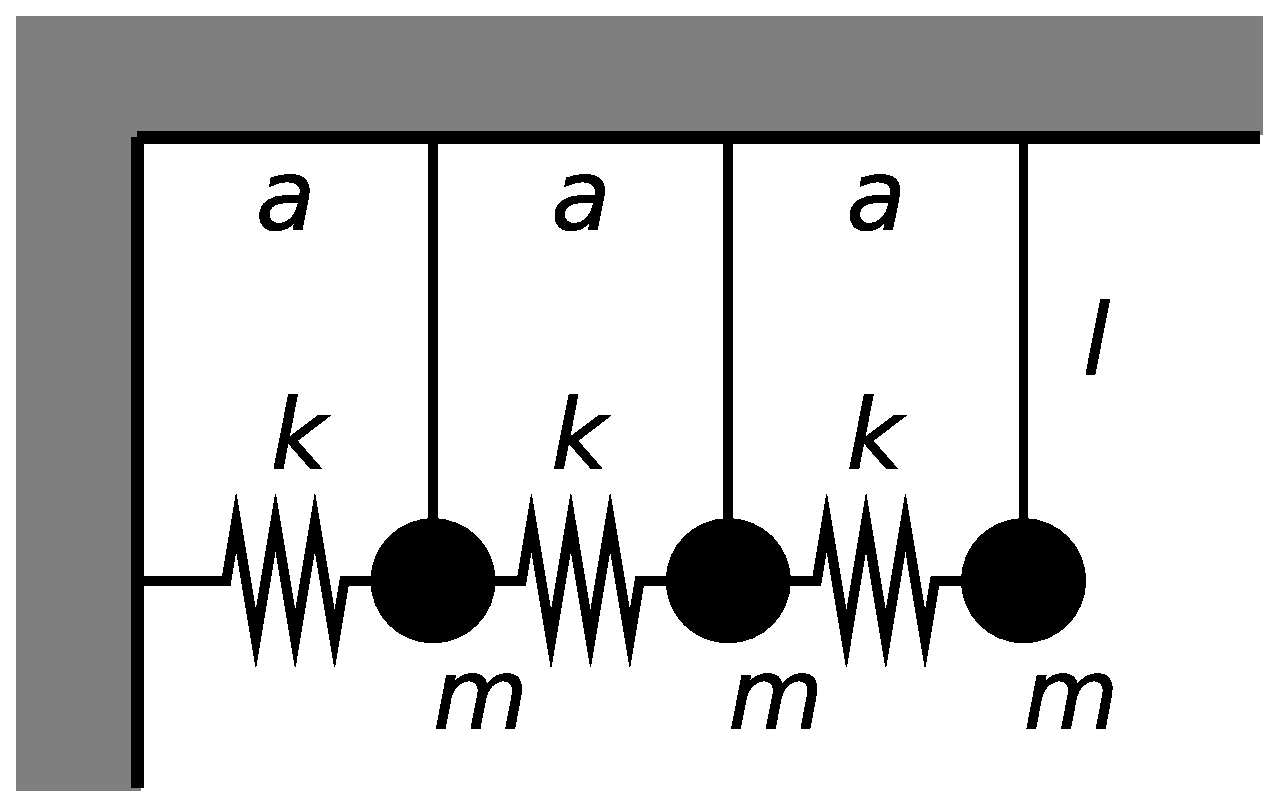
\includegraphics[width=\textwidth]{ej1-14}
%\end{minipage}
